\documentclass{standalone}
\usepackage{tikz}
\usepackage{ctex,siunitx}
\setCJKmainfont{Noto Serif CJK SC}
\usepackage{tkz-euclide}
\usepackage{amsmath}
\usetikzlibrary{patterns, calc}
\usetikzlibrary {decorations.pathmorphing, decorations.pathreplacing, decorations.shapes,}

\begin{document}
\small
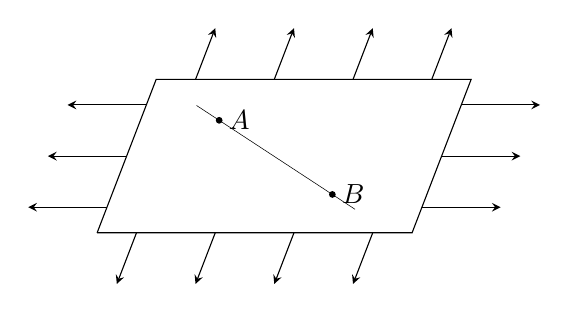
\begin{tikzpicture}[>=stealth,yscale=1.5, x={(0:1cm)}, y={(60:.5cm)}]
  \tkzSetUpPoint[fill=black]
  % \useasboundingbox(-1,-0.75)rectangle(3.7,1.4);

  \draw (0,0)--(4,0)--(4,3)--(0,3)--(0,0);
  \foreach \x in {.5,1.5,...,3.5}
  {
    \draw[->](\x,0)--(\x,-1);
    \draw[->](\x,3)--(\x,4);
  }
  \foreach \x in {.5,1.5,2.5}
  {
    \draw[->](0,\x)--(-1,\x);
    \draw[->](4,\x)--(5,\x);
  }
  
  \tkzDefPoints{1/2.2/A, 2.8/.75/B}
  \tkzDrawLine(A,B)
  \tkzDrawPoints(A,B)
  \tkzLabelPoints[right](A,B)		
\end{tikzpicture}
\end{document}